\chapter{Persona's}
    \label{personasappendix}
De onderstaande persona's zijn gebaseerd op de interne doelgroepanalyse van Wakoopa en de gegevens uit de uitgevoerde Enqu\^ete.

\section{Tom Daaler}
  \begin{wrapfigure}{l}{40mm}
      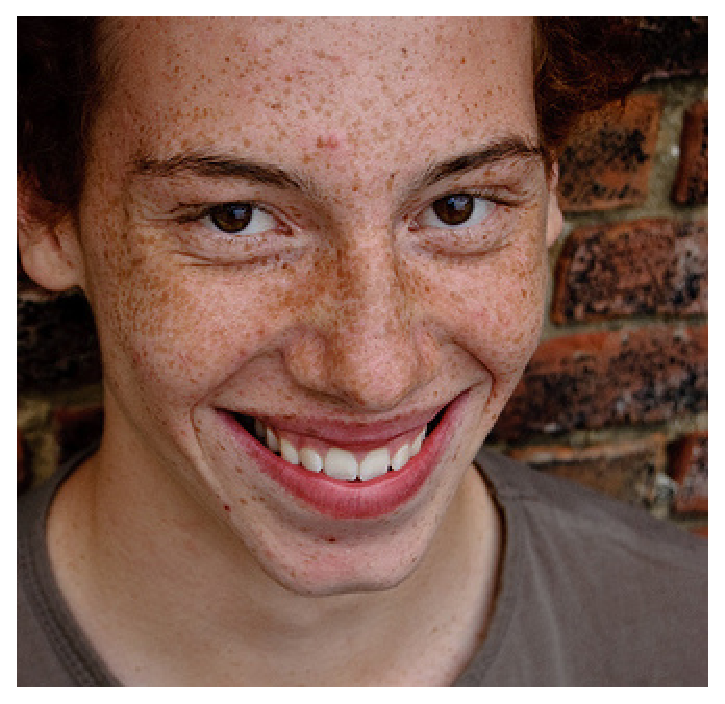
\includegraphics[height=40mm]{../images/personas/tom}
  \end{wrapfigure}
Tom is 17 jaar en zit in zijn laatste jaar havo. Hij werkt als vakkenvuller bij de AH en spendeert het meeste van zijn vrije tijd achter de pc waar hij games speelt of zijn pc aan het tweaken is. Het geld wat hij bij de AH verdient gaat voornamelijk op aan games en hardware. Hij is nieuwsgierig en probeert daarom vaak nieuwe programma's. Wanneer hij een nieuw programma ontdekt is hij vaak een van de eerste onder zijn vrienden, en is trots als hij zijn bevindingen kan delen en aan anderen kan uitleggen hoe een nieuw programma werkt.

In het MBTI model zoals gebruikt in \cite{Klompsma} is Tom een competetieve bezoeker.

\section{Andreas Nilsson}
  \begin{wrapfigure}{l}{40mm}
      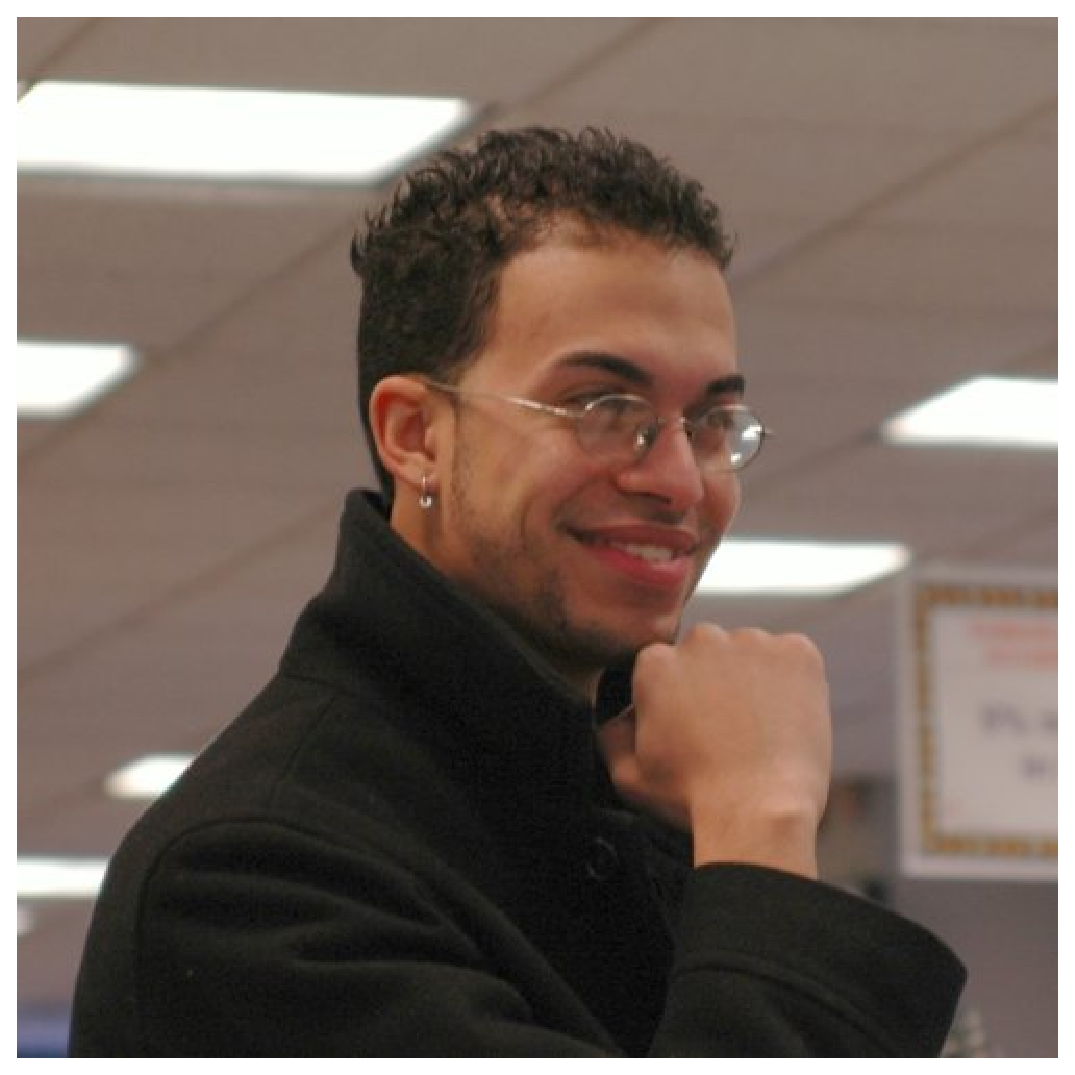
\includegraphics[height=40mm]{../images/personas/andreas}
  \end{wrapfigure}
Andreas is 28 jaar en heeft een baan bij een IT-bedrijf als programmeur. Buiten zijn werk probeert hij de computer te ontwijken, hoewel hij 's avonds vaak nog even op Youtube of Hyves zit. Hij wil graag zo effici\"ent mogelijk werken en ergert zich snel aan programma's. Daarentegen wilt hij ook niet te veel tijd besteden aan het vinden en uitzoeken van nieuwe programma's. Het is voor hem belangrijk dat hij zo goed mogelijk zijn werk kan doen en daarbij niet te veel aan andere dingen hoeft te denken. Andreas moet van zijn bedrijf bijhouden waar zijn tijd aan opgaat, iets waar hij eigenlijk niet op zit te wachten.

In het MBTI model zoals gebruikt in \cite{Klompsma} is Andreas een competetieve bezoeker.

\section{Johan Broers}
  \begin{wrapfigure}{l}{40mm}
      
\includegraphics[height=40mm]{../images/personas/johan}
  \end{wrapfigure}
Johan is 32 en de maker van TimeSink, een klein programma om je tijd te managen. Hiervan heeft hij een gratis versie en een betaalde versie met meer opties. Naast dit programma werkt hij zelf als freelancer voor verschillende softwarebedrijven, maar het liefst zou hij genoeg verdienen om eigen baas te kunnen worden. Hij komt graag in contact met gebruikers van zijn programma en is zeer ge\"interesseerd in wat ze van zijn programma vinden. Hij kijkt vaak naar zijn downloadstatistieken, maar blijft benieuwd naar hoeveel mensen zijn programma nou echt gebruiken.

In het MBTI model zoals gebruikt in \cite{Klompsma} is Johan een humanistische bezoeker.

\section{Mari\"ette Klompman}
  \begin{wrapfigure}{l}{40mm}
      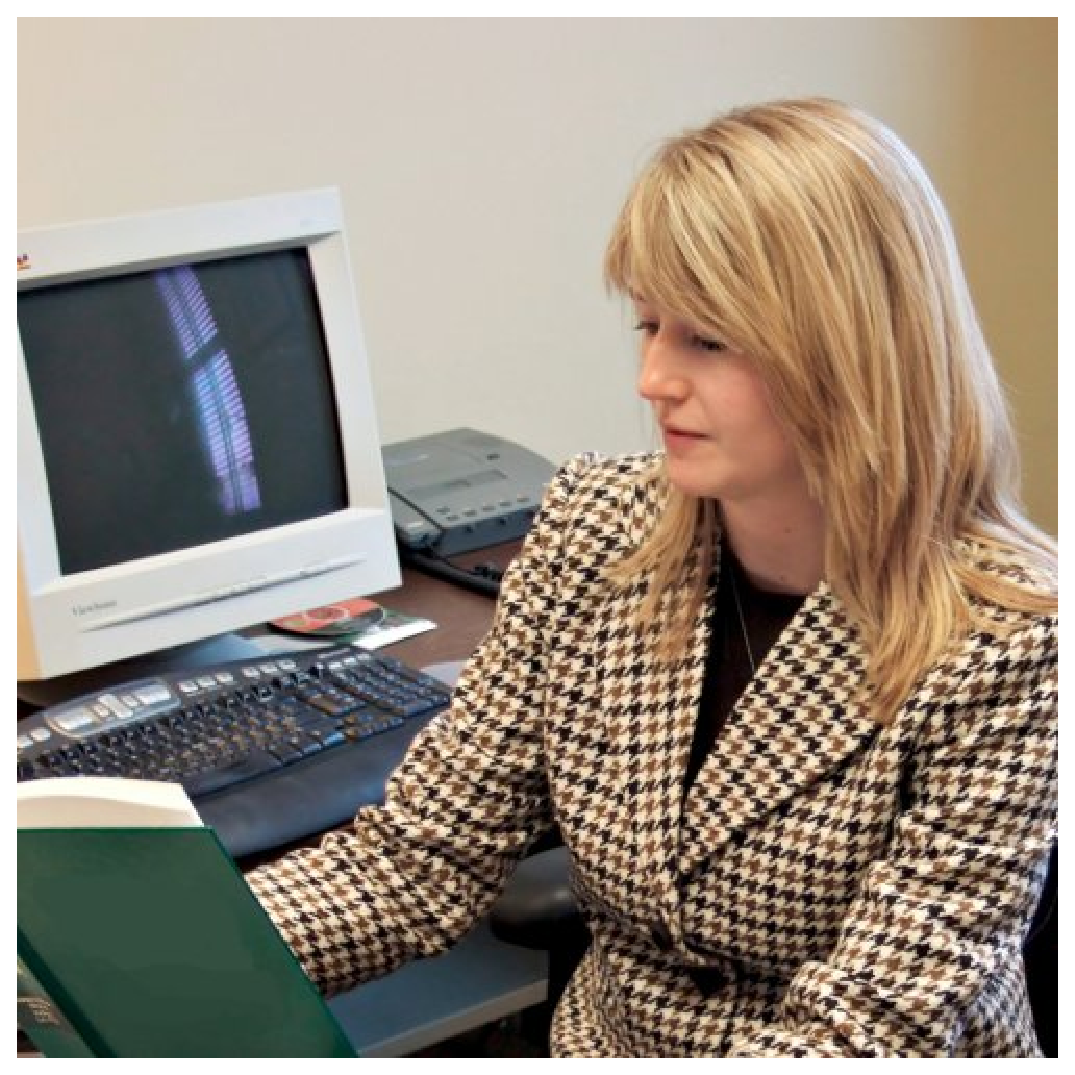
\includegraphics[height=40mm]{../images/personas/mariette}
  \end{wrapfigure}
Mari\"ette is een administratief medewerker voor een scholengemeenschap en moeder van 2 kinderen van 8 en 5. Voor haar werk zit ze veel in Microsoft Office, maar thuis doet ze eigelijk niks met de computer. In haar vrije tijd loopt ze hard en schildert ze. Ze is niet heel vaardig met de computer, ondanks dat ze voor haar werk een cursus office en internet heeft gevolgd. Soms loopt ze vast met Word, en vraagt dan haar collega om hulp. Op dagen dat haar collega er niet is, probeerd ze via Google toch het antwoord te vinden, maar vaak vind ze niet wat ze zoekt, of ze snapt de gebruikte termen niet helemaal. Als ze het niet snel kan vinden schrijft ze het om op later aan haar collega te vragen en gaat dan ergens anders mee verder.

In het MBTI model zoals gebruikt in \cite{Klompsma} is Mariette een spontane bezoeker.

